\documentclass[14pt]{extreport}
\usepackage{gost}

%Тут можно вставить дополнительные пакеты

\begin{document}
\pagestyle{empty} %  выключаем нумерацию
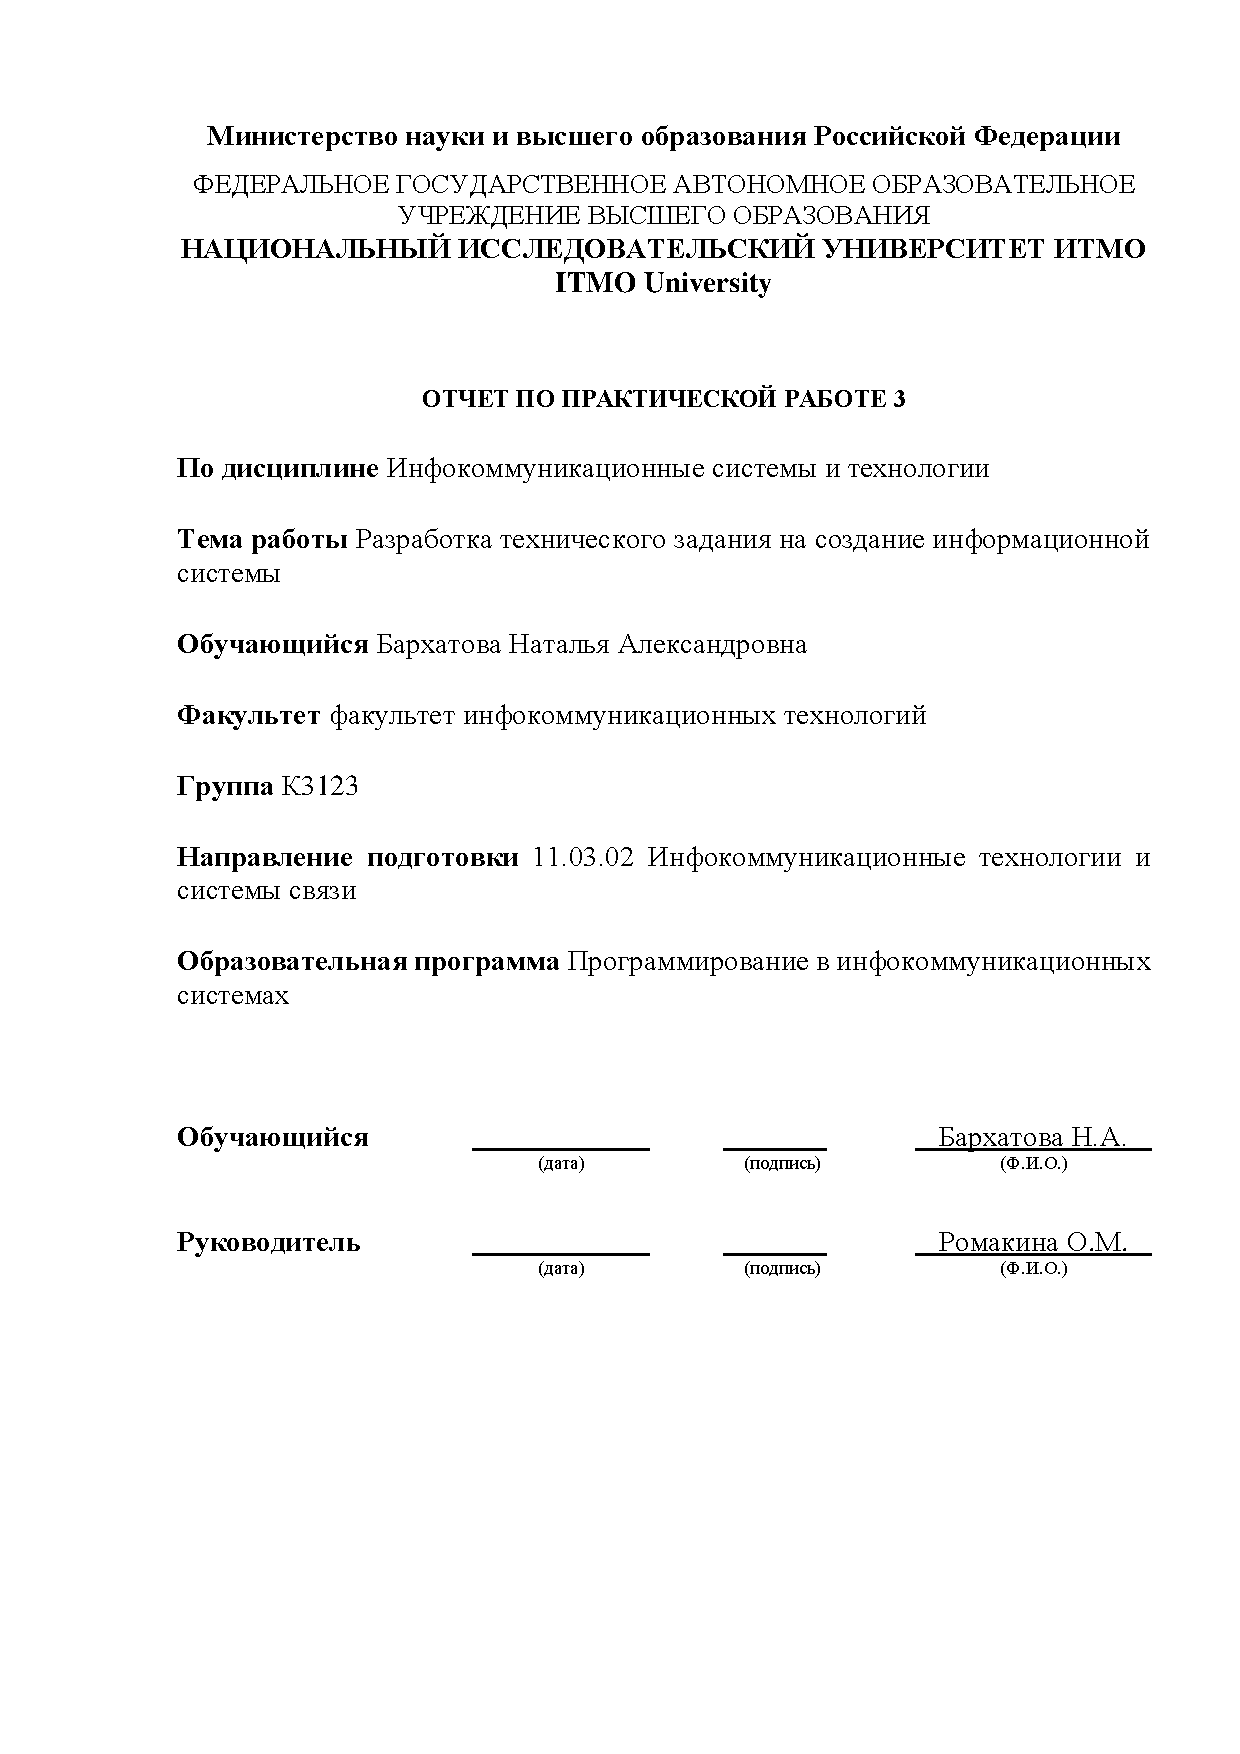
\includepdf[pages=-,pagecommand={}]{PR3Title.pdf}
\pagestyle{plain} % включаем нумерацию

\tableofcontents

\intro

В данном отчете описаны основные моменты будущего мобильного приложения: название, назначение, анализ основных пользователей системы, планируемый набор функций для каждого из будущих пользователей, прототип интерфейса будущей системы, обзор аналогов, представленных на рынке и обоснование необходимости разработки данного мобильного приложения.

\chapter{ОСНОВНАЯ ЧАСТЬ}

Мобильное приложение \textbf{\textit{"My food"}} предназначно для анализа количества продуктов, контроля срока годности продуктов и подбора рецетов, основываясь на наличии требуемых ингридиентов в холодильнике.

Основными пользователями системы являются: 
\begin{itemize}
    \item 1 категория: обычные потребители продовольственных товаров
    \item 2 категория: пользователи, увлекающиеся кулинарией
    \item 3 категория: пользователи, тщательно следящие за своим питанием
\end{itemize}
\textit{Замечание}: пользователь может относиться к нескольким категориям одновременно

\section{Планируемый набор функций для пользователей 1 категории: }

\begin{enumerate}
    \item \textbf{Добавить продукт в холодильник} 
    \newline
    Возможность добавления купленных продуктов в виртуальный холодильным посредством \textbf{сканирования штрих-кода товара}, ручного ввода (в случае невозможности сканирования). В базу данных виртуального холодильника вносится информация о типе товара (фрукты/овощи, хлебобулочные изделия, молочная продукция, бакалея, мясные и колбасные изделия, рыба, кондитерские изделия), объеме товара (штуки, граммы, литры) и оставшемся сроке годности.
    \item \textbf{Подходящий срок годности продукта}
    \newline
    В случае обнаружения в базе данных продуктов, срок годности которых подходит к концу (2-3 дня) или истёк, приложение сообщает пользователю об этом.
    \item \textbf{Список продуктов} 
    \newline
    В данном списке отображаются продукты (полная база данных), разделенные по типам. 
    \item \textbf{Список покупок} 
    \newline
    Пользователь имеет возможность составлять список покупок для похода в магазин. Приложение рекомендует пользователю добавить в список продукты первой необходимости, которые закончились в <<холодильнике>>.
    \item \textbf{Многопользовательский режим (<<Семья>>)} 
    \newline 
    Если пользователь разделяет продукты в холодильнике с другим человеком, существует возможность <<Добавить в семью>>, то есть подключить другого пользователя приложения к своему <<виртуальному холодильнику>>. Таким образом все члены <<Семьи>> будут иметь возможность добавлять/удалять продукты из базы данных холодильника. Однако, каждый пользователь всё ещё может настроивать личную диету.
    
\end{enumerate}
\section {Планируемый набор функций для пользователей 2 категории: }
\begin{enumerate}
    \item \textbf{Предлагаемые рецепты. Книга рецептов} 
    \newline
    Основываясь на перечне продуктов в базе данных виртуального холодильника, приложение отбирает из книги рецептов те блюда, которые можно приготовить из имеющегося набора продуктов. Если пользователь выбирает рецепт, то из <<виртуального холодильника>> автоматичестки удаляются продукты, входящие в состав рецепта.
\end{enumerate}
\section {Планируемый набор функций для пользователей 3 категории: }
\begin{enumerate}
    \item \textbf{Выбор диеты} 
    \newline
    В режиме определенной диеты приложение анализирует каждый продукт в <<холодильнике>> на допустимость к употреблению пользователем. В списке продуктов не рекомендуемые товары подсвечиваются красным, когда как рекомендуемые - зелёным. Рекоммендательная система рецептов также подстраивается под диету пользователя.
    \item \textbf{Статистика пользователя}
    \newline
    На основе данных потребления продуктов составляется недельный отчёт о питании пользователя. Продукты разделены по типам. Ведётся посчет употребленных в день каллорий, белков, жиров и углеводов. Приложение анализирует статистику веществ и на основе выбранной диеты делает рекомендации.
\end{enumerate}
\newpage
\chapter{ОБЗОР АНАЛОГОВ}

\section{Приложение из Google Play <<Учёт продуктов, Список покупок>>\cite{bib1}}
\begin{enumerate}
\item ОСНОВНЫЕ ФУНКЦИИ: это приложение позволяет вести учет продуктов у пользователя дома и отслеживать их сроки годности. Пользователь также может добавлять продукты в список покупок, а после покупки добавлять их в список продуктов, хранящихся дома. Для удобства пользователь может рассортировать продукты по группам и определить места хранения, чтобы знать, где, что и в каком количестве лежит. Для более быстрой работы можно сканировать штрих-коды. Пользователь может работать со списками с любого своего устройства и открыть доступ своим родственникам или друзьям для совместного использования. 

\item ТАРИФЫ: 
базовое приложение бесплатное, премиум-версия стоит 59 р/мес (или 500 р/год). В премеум-версию входят следующие функции: <<Добавление других полователей для совместного использования и синхронизации списков>> и <<Установка индивидуальных сроков предупреждений для категорий продуктов>>.

\item ПРЕИМУЩЕСТВА: 
\begin{enumerate}
    \item Есть возможность сканирования штрих-кодов
    \item Удобный и понятный интерфейс
    \item Напоминание о сроке годности
    \item Облачная синхронизация
    \item Возможность совместного использования приложения
\end{enumerate}

\itemНЕДОСТАТКИ: 
\begin{enumerate}
    \item Небольшой набор функций
    \item Доступно только на Android
    \item Наличие крупных баннеров с рекламой в базовой версии.
\end{enumerate}

\itemОБЩИЕ ВЫВОДЫ: 

Данное приложение удобно в использовании, оно хорошо подойдет для контроля продуктов. Однако, введение премиум версии неоправданно всего для двух дополнительных функций, которые не сильно изменят мнение о приложении. Возможность сканирования штрих-кодов позволяет сильно экономить время, что несомненно является большим преимуществом.
\end{enumerate}
\section{Приложение из Google Play <<Wonder Fridge>>\cite{bib2}}
\begin{enumerate}
\item ОСНОВНЫЕ ФУНКЦИИ: данное приложение включает в себя следующие функции: добавление продуктов вручную (либо выбрав нужный продукт из списка предложенных), возможность задавать срок годности продукта, разделение продуктов на <<Холодильник>>, <<Морозилку>> и <<Кладовку>>, наличие списка покупок. Приложение напоминает пользователю об истекшем сроке годности продукта. Доступно резервное копирование/восстановление данных.

\item ТАРИФЫ: платными являются только косметические элементы.
\item ПРЕИМУЩЕСТВА: 
\begin{enumerate}
    \item Приложение присылает напоминание о сроке годности
    \item Присутствует разделение продуктов на типы
    \item Вполне удобный и приятный интерфейс
    \item Есть возможность добавлять продукты из списка предложенных
\end{enumerate}

\item НЕДОСТАТКИ: 
\begin{enumerate}
    \item Нет возможности сканирования штрих-кодов
    \item Доступно только на Android
    \item Небольшой набор функций
    \item Некачественная локализация на русский язык (много опечаток и кусков вовсе не переведенного текста)
\end{enumerate}
\item ОБЩИЕ ВЫВОДЫ: 

Данное приложение имеет всего две основных функции, однако реализованные достаточно качественно. Отсутствие сканера штрих-кодов компенсируется удобным списком предлагаемых продуктов. <<Wonder Fridge>> является хорошим приложением с узкой специализацией. Однако, некачественная локализация сильно портит впечатление.
\end{enumerate}
\section{Приложение из Google Play <<SuperCook Поисковик Рецептов>>\cite{bib3}}
\begin{enumerate}
\item ОСНОВНЫЕ ФУНКЦИИ: данное приложение анализирует огромное множество рецептов со всего инетернета и предлагает пользователю только те, которые он может приготовить из имеющихся у него ингридиентов. Для этого пользователю необходимо дать разрешение на доступ к микрофону и начать перечислять вслух все продукты. SuperCook автоматически подберет рекомендации блюд к приготовлению. Мен. <<рецепты>> для удобства разбито на несколько категорий, таких как <<Салаты>>, <<Супы>>, <<Закуски>>, <<Десерты>> и многое другое.
\item ТАРИФЫ: приложение полностью бесплатное

\item ПРЕИМУЩЕСТВА: 

\begin{enumerate}
    \item Возможность вводить перечень продуктов с помощью голоса
    \item Присутствует разделение продуктов на типы
    \item Вполне удобный и приятный интерфейс
    \item Облачная синхронизация
    \item Эффективный подбор рецептов
\end{enumerate}

\item НЕДОСТАТКИ: 
\begin{enumerate}
    \item Много лишней информации на главной странице приложения
    \item Доступно только на Android
    \item Не учитывается количество имеющихся продуктов
\end{enumerate}
\item ОБЩИЕ ВЫВОДЫ: 

<<SuperCook>> не очень удобен в использовании, так как он, во-первых, не учитывает срок годности продуктов, к тому моменту, когда пользователь выбрал рецепт, ингридиент уже может быть испорчен, но всё еще остаётся в базе данных и учитывается при подборе рецептов. Во-вторых, в приложении не учитывается количество нужного для претворения рецепта в жизнь ингридиента (к примеру, у пользователя может быть 0.3 литра молока в наличии, но для рецепта нужен 1 литр).  Идея приложения очень хорошая, но при реализации возникли мелкие проблемы, портящие впечатление о приложении в целом.
\end{enumerate}
\newpage
\chapter{ПРОТОТИП}

Прототип создан с помощью Figma. \cite{bib4}
\begin{figure}[H]
\centerline{\includegraphics[width=0.5\linewidth]{Untitled (1)-1.png}}
\caption{Список продуктов в холодильнике}
\label{r1}
\end{figure}

\begin{figure}[H]
\centerline{\includegraphics[width=0.5\linewidth]{Untitled (1)-2.png}}
\caption{Список покупок}
\label{r2}
\end{figure}

\begin{figure}[H]
\centerline{\includegraphics[width=0.5\linewidth]{Untitled (1)-3.png}}
\caption{Предлагаемые рецепты. Книга рецептов}
\label{r3}
\end{figure}

\begin{figure}[H]
\centerline{\includegraphics[width=0.5\linewidth]{Untitled (1)-4.png}}
\caption{Выбор рецепта}
\label{r4}
\end{figure}
\conclusions

Была разработана идея приложения <<My food>>, описаны основные пользователи приложения а также основные функции. Пронализировав аналоги на рынке, выяснилось, что запланированное приложение <<My food>> включает в себя функции, частично реализованные в аналогах. Однако аналоги представляют собой узкоспециализированные приложения, имеющие существенные минусы. Таким образом, разработка приложения <<My food>> оправдана и необходима.
\newpage
\begin{thebibliography}{}
\bibitem{bib1} Учет Продуктов, Список Покупок [Электронный ресурс]:  приложение, позволяющее вести учет продуктов у вас дома и отслеживать их сроки годности. – Режим доступа: \url{https://play.google.com/store/apps/details?id=com.chestersw.foodlist} (дата обращения: 23.10.2022).
\bibitem{bib2} Wonder Fridge: Холодильник [Электронный ресурс]:  приложение, позволяющее следить за продуктами в холодильнике. – Режим доступа: \url{https://play.google.com/store/apps/details?id=com.meolly.fridge} (дата обращения: 23.10.2022).
\bibitem{bib3} SuperCook Поисковик рецептов [Электронный ресурс]:  Рецепты из того, что есть дома. – Режим доступа: \url{https://play.google.com/store/apps/details?id=com.supercook.app} (дата обращения: 23.10.2022).
\bibitem{bib4} Figma [Электронный ресурс]: Графический онлайн-редактор для совместной работы. – Режим доступа: \url{https://www.figma.com/} (дата обращения: 19.10.2022)
\end{thebibliography}
\end{document}
\end{document}
